%!TEX TS-program = xelatex

% Шаблон документа LaTeX создан в 2018 году
% Алексеем Подчезерцевым
% В качестве исходных использованы шаблоны
% 	Данилом Фёдоровых (danil@fedorovykh.ru) 
%		https://www.writelatex.com/coursera/latex/5.2.2
%	LaTeX-шаблон для русской кандидатской диссертации и её автореферата.
%		https://github.com/AndreyAkinshin/Russian-Phd-LaTeX-Dissertation-Template

\documentclass[a4paper,14pt]{article}


%%% Работа с русским языком
\usepackage[english,russian]{babel}   %% загружает пакет многоязыковой вёрстки
\usepackage{fontspec}      %% подготавливает загрузку шрифтов Open Type, True Type и др.
\defaultfontfeatures{Ligatures={TeX},Renderer=Basic}  %% свойства шрифтов по умолчанию
\setmainfont[Ligatures={TeX,Historic}]{Times New Roman} %% задаёт основной шрифт документа
\setsansfont{Comic Sans MS}                    %% задаёт шрифт без засечек
\setmonofont{Courier New}
\usepackage{indentfirst}
\frenchspacing

\renewcommand{\epsilon}{\ensuremath{\varepsilon}}
\renewcommand{\phi}{\ensuremath{\varphi}}
\renewcommand{\kappa}{\ensuremath{\varkappa}}
\renewcommand{\le}{\ensuremath{\leqslant}}
\renewcommand{\leq}{\ensuremath{\leqslant}}
\renewcommand{\ge}{\ensuremath{\geqslant}}
\renewcommand{\geq}{\ensuremath{\geqslant}}
\renewcommand{\emptyset}{\varnothing}

%%% Дополнительная работа с математикой
\usepackage{amsmath,amsfonts,amssymb,amsthm,mathtools} % AMS
\usepackage{icomma} % "Умная" запятая: $0,2$ --- число, $0, 2$ --- перечисление

%% Номера формул
%\mathtoolsset{showonlyrefs=true} % Показывать номера только у тех формул, на которые есть \eqref{} в тексте.
%\usepackage{leqno} % Нумерация формул слева	

%% Перенос знаков в формулах (по Львовскому)
\newcommand*{\hm}[1]{#1\nobreak\discretionary{}
	{\hbox{$\mathsurround=0pt #1$}}{}}

%%% Работа с картинками
\usepackage{graphicx}  % Для вставки рисунков
\graphicspath{{images/}}  % папки с картинками
\setlength\fboxsep{3pt} % Отступ рамки \fbox{} от рисунка
\setlength\fboxrule{1pt} % Толщина линий рамки \fbox{}
\usepackage{wrapfig} % Обтекание рисунков текстом

%%% Работа с таблицами
\usepackage{array,tabularx,tabulary,booktabs} % Дополнительная работа с таблицами
\usepackage{longtable}  % Длинные таблицы
\usepackage{multirow} % Слияние строк в таблице
\usepackage{float}% http://ctan.org/pkg/float

%%% Программирование
\usepackage{etoolbox} % логические операторы


%%% Страница
\usepackage{extsizes} % Возможность сделать 14-й шрифт
\usepackage{geometry} % Простой способ задавать поля
\geometry{top=20mm}
\geometry{bottom=20mm}
\geometry{left=20mm}
\geometry{right=10mm}
%
%\usepackage{fancyhdr} % Колонтитулы
% 	\pagestyle{fancy}
%\renewcommand{\headrulewidth}{0pt}  % Толщина линейки, отчеркивающей верхний колонтитул
% 	\lfoot{Нижний левый}
% 	\rfoot{Нижний правый}
% 	\rhead{Верхний правый}
% 	\chead{Верхний в центре}
% 	\lhead{Верхний левый}
%	\cfoot{Нижний в центре} % По умолчанию здесь номер страницы

\usepackage{setspace} % Интерлиньяж
\onehalfspacing % Интерлиньяж 1.5
%\doublespacing % Интерлиньяж 2
%\singlespacing % Интерлиньяж 1

\usepackage{lastpage} % Узнать, сколько всего страниц в документе.

\usepackage{soul} % Модификаторы начертания

\usepackage{hyperref}
\usepackage[usenames,dvipsnames,svgnames,table,rgb]{xcolor}
\hypersetup{				% Гиперссылки
	unicode=true,           % русские буквы в раздела PDF
	pdftitle={Практическая по БД},   % Заголовок
	pdfauthor={Подчезерцев Алексей},      % Автор
	pdfsubject={Создание и заполнение отношений БД фитнес-клуба},      % Тема
	pdfcreator={Подчезерцев Алексей}, % Создатель
	pdfproducer={Подчезерцев Алексей}, % Производитель
	pdfkeywords={БД} {SQL} {MySQL}, % Ключевые слова
	colorlinks=true,       	% false: ссылки в рамках; true: цветные ссылки
	linkcolor=black,          % внутренние ссылки
	citecolor=black,        % на библиографию
	filecolor=magenta,      % на файлы
	urlcolor=black           % на URL
}
\makeatletter 
\def\@biblabel#1{#1. } 
\makeatother
\usepackage{cite} % Работа с библиографией
%\usepackage[superscript]{cite} % Ссылки в верхних индексах
%\usepackage[nocompress]{cite} % 
\usepackage{csquotes} % Еще инструменты для ссылок

\usepackage{multicol} % Несколько колонок

\usepackage{tikz} % Работа с графикой
\usepackage{pgfplots}
\usepackage{pgfplotstable}

% ГОСТ заголовки
\usepackage[font=small]{caption}
%\captionsetup[table]{justification=centering, labelsep = newline} % Таблицы по правобу краю
%\captionsetup[figure]{justification=centering} % Картинки по центру


\newcommand{\tablecaption}[1]{\addtocounter{table}{1}\small \begin{flushright}\tablename \ \thetable\end{flushright}%	
\begin{center}#1\end{center}}

\newcommand{\imref}[1]{Рис.~\ref{#1}}

\usepackage{multirow}
\usepackage{spreadtab}
\newcolumntype{K}[1]{@{}>{\centering\arraybackslash}p{#1cm}@{}}


\usepackage{xparse}
\ExplSyntaxOn
\DeclareExpandableDocumentCommand{\juliandate}{ m m m }
{
	\juliandate_calc:nnnn { #1 } { #2 } { #3 } { \use:n }
}
\NewDocumentCommand{\storejuliandate}{ s m m m m }
{
	\IfBooleanTF{#1}
	{
		\juliandate_calc:nnnn { #3 } { #4 } { #5 } { \cs_set:Npx #2 }
	}
	{
		\juliandate_calc:nnnn { #3 } { #4 } { #5 } { \cs_new:Npx #2 }
	}
}
\cs_new:Npn \juliandate_calc:nnnn #1 #2 #3 #4 % #1 = day, #2 = month, #3 = year, #4 = what to do
{
	#4 
	{
		\int_eval:n
		{
			#1 +
			\int_div_truncate:nn { 153 * (#2 + 12 * \int_div_truncate:nn { 14 - #2 } { 12 } - 3) + 2 } { 5 } +
			365 * (#3 + 4800 - \int_div_truncate:nn { 14 - #2 } { 12 } ) +
			\int_div_truncate:nn { #3 + 4800 - \int_div_truncate:nn { 14 - #2 } { 12 } } { 4 } -
			\int_div_truncate:nn { #3 + 4800 - \int_div_truncate:nn { 14 - #2 } { 12 } } { 100 } + 
			\int_div_truncate:nn { #3 + 4800 - \int_div_truncate:nn { 14 - #2 } { 12 } } { 400 } -
			32045
		}
	}
}

\tl_new:N \l__juliandate_g_tl
\tl_new:N \l__juliandate_dg_tl
\tl_new:N \l__juliandate_c_tl
\tl_new:N \l__juliandate_dc_tl
\tl_new:N \l__juliandate_b_tl
\tl_new:N \l__juliandate_db_tl
\tl_new:N \l__juliandate_a_tl
\tl_new:N \l__juliandate_da_tl
\tl_new:N \l__juliandate_y_tl
\tl_new:N \l__juliandate_m_tl
\tl_new:N \l__juliandate_d_tl
\int_new:N \l_juliandate_day_int
\int_new:N \l_juliandate_month_int
\int_new:N \l_juliandate_year_int

\cs_new:Npn \__juliandate_set:nn #1 #2
{
	\tl_set:cx { l__juliandate_#1_tl } { \int_eval:n { #2 } }
}
\cs_new:Npn \__juliandate_use:n #1
{
	\tl_use:c { l__juliandate_#1_tl }
}
\cs_new_protected:Npn \juliandate_reverse:n #1
{
	\__juliandate_set:nn { g }
	{ \int_div_truncate:nn { #1 + 32044 } { 146097 } }
	\__juliandate_set:nn { dg }
	{ \int_mod:nn { #1 + 32044 } { 146097 } }
	\__juliandate_set:nn { c }
	{ \int_div_truncate:nn { ( \int_div_truncate:nn { \__juliandate_use:n { dg } } { 36524 } + 1) * 3 } { 4 } }
	\__juliandate_set:nn { dc }
	{ \__juliandate_use:n { dg } - \__juliandate_use:n { c } * 36524 }
	\__juliandate_set:nn { b }
	{ \int_div_truncate:nn { \__juliandate_use:n { dc } } { 1461 } }
	\__juliandate_set:nn { db }
	{ \int_mod:nn { \__juliandate_use:n { dc } } { 1461 } }
	\__juliandate_set:nn { a }
	{ \int_div_truncate:nn { ( \int_div_truncate:nn { \__juliandate_use:n { db } } { 365 } + 1) * 3 } { 4 } }
	\__juliandate_set:nn { da }
	{ \__juliandate_use:n { db } - \__juliandate_use:n { a } * 365 }
	\__juliandate_set:nn { y }
	{
		\__juliandate_use:n { g } * 400 + 
		\__juliandate_use:n { c } * 100 + 
		\__juliandate_use:n { b } * 4 + 
		\__juliandate_use:n { a }
	}
	\__juliandate_set:nn { m }
	{ \int_div_truncate:nn { \__juliandate_use:n { da } * 5 + 308 } { 153 } - 2 }
	\__juliandate_set:nn { d }
	{ \__juliandate_use:n { da } - \int_div_truncate:nn { (\__juliandate_use:n { m } + 4) * 153 } { 5 } + 122 }
	\int_set:Nn \l_juliandate_year_int
	{ \__juliandate_use:n { y } - 4800 + \int_div_truncate:nn { \__juliandate_use:n { m } + 2 } { 12 } }
	\int_set:Nn \l_juliandate_month_int
	{ \int_mod:nn { \__juliandate_use:n { m } + 2 } { 12 } + 1 }
	\int_set:Nn \l_juliandate_day_int
	{ \__juliandate_use:n { d } + 1 }
}
\cs_generate_variant:Nn \juliandate_reverse:n { x }

\NewDocumentCommand{\showday}{ m }
{
	\juliandate_reverse:n { #1 }
	\int_to_arabic:n { \l_juliandate_day_int }-
	\int_to_arabic:n { \l_juliandate_month_int }-
	\int_to_arabic:n { \l_juliandate_year_int }
}

\NewDocumentCommand{\tomorrow}{ }
{
	\group_begin:
	\juliandate_reverse:x { \juliandate_calc:nnnn { \day + 1 } { \month } { \year } { \use:n } }
	\day = \l_juliandate_day_int
	\month = \l_juliandate_month_int
	\year = \l_juliandate_year_int
	\today
	\group_end:
}
\NewDocumentCommand{\tomorrowof}{ m m m }
{
	\group_begin:
	\juliandate_reverse:x { \juliandate_calc:nnnn { #1 + 1 } { #2 } { #3 } { \use:n } }
	\day = \l_juliandate_day_int
	\month = \l_juliandate_month_int
	\year = \l_juliandate_year_int
	\today
	\group_end:
}
\ExplSyntaxOff


\usepackage{xcolor,listings}
\usepackage{textcomp}
\begin{document} % конец преамбулы, начало документа
\begin{titlepage}
	\begin{center}
		ФЕДЕРАЛЬНОЕ  ГОСУДАРСТВЕННОЕ АВТОНОМНОЕ \\
		ОБРАЗОВАТЕЛЬНОЕ УЧРЕЖДЕНИЕ ВЫСШЕГО ОБРАЗОВАНИЯ\\
		«НАЦИОНАЛЬНЫЙ ИССЛЕДОВАТЕЛЬСКИЙ УНИВЕРСИТЕТ\\
		«ВЫСШАЯ ШКОЛА ЭКОНОМИКИ»
	\end{center}
	
	\begin{center}
		\textbf{Московский институт электроники и математики}
		
		\textbf{Им. А.Н.Тихонова НИУ ВШЭ}
		
		\textbf{Департамент электронной инженерии}
	\end{center}	
	\vspace{5ex}
	\begin{center}
\textbf{<<ПОЛУЧЕНИЕ, ОБРАБОТКА И ПРЕДСТАВЛЕНИЕ РЕЗУЛЬТАТОВ МНОГОКРАТНЫХ ИЗМЕРЕНИЙ>>}
	\end{center}	
	\vspace{1ex}
	\begin{center}
\textbf{Отчёт по части 2 лабораторного практикума по дисциплине \\
	<<Электротехника, электроника и метрология>>, раздел <<Метрология>>(ЛР 5-7)}
	\end{center}	
	\vspace{5ex}
	
	\begin{multicols}{2}
	\vfill\null
	\columnbreak
	ВЫПОЛНИЛИ:
	
	Подчезерцев Алексей Евгеньевич
	
	Солодянкин Андрей Александрович
	
	группа БИВ172
	\end{multicols}

	\vfill
	\begin{center}
		Москва \the\year
	\end{center}
\end{titlepage}
\tableofcontents
\pagebreak
\section{Цель работы}

\begin{itemize}
	\item Изучение статических вольт-амперных характеристик МДП транзистора;
	\item Изучение способов и определение параметров его модели для схемотехнических расчетов
	\item Приобретение навыков работы с полупроводниковыми приборами;
	\item Приобретение навыков расчета схем с помощью SРIСЕ-симулятора.
\end{itemize}

\section{Теоретическое введение}

\subsection{Общие сведения}

МДП-транзистор - одна из разновидностей униполярного (полевого)
транзистора. Суть любого полевого транзистора состоит в следующем : в его
основе лежит проводящий канал с двумя контактами, называемыми сток
и исток; концентрация же носителей заряда в канале (а значит и электрическая
проводимость канала) управляется электрическим полем, возникающим
при подаче напряжения на третий вывод, называемый затвором. Отсюда
и название всех полевых транзисторов.

Особенностью МДП-транзисторов является то, что в них затвор отделён
от проводящего канала слоем диэлектрика, так что управляющая структура
такого транзистора составлена из слоёв Металла - Диэлектрика - Полупроводника
(МДП). МДП-транзистор, таким образом, - это полевой транзистор
с изолированным затвором - он представляет собой полупроводниковый
прибор, работа которого основана на использовании эффекта поля в структуре
металл-диэлектрик-полупроводник. В том распространённом частном
случае, когда в качестве диэлектрика применяется оксид кремния SiO 2, используется
название МОП-транзистор (МОПТ, Metal-Oxide-Semiconductor 
Field Effect Transistor - MOSFET). В современных транзисторах вместо SiO 2
нередко используются другие материалы с большей диэлектрической проницаемостью
(на основе гафния, циркония, тантала и др.), а в качестве материала
затвора поликремний, однако закрепившееся название «МОП-транзистор»
распространяется и на эти структуры.

Работа всех униполярных транзисторов, и в том числе МОПТ, основана
на использовании только одного типа носителей - основных (или электронов,
или дырок); процессы инжекции и диффузии в таких транзисторах не играют
принципиальной роли. Основным способом движения носителей является
дрейф в электрическом поле. Отметим, что в современных нанометровых
МОП-транзисторах подзатворный диэлектрик настолько тонкий, что сквозь
него возможно туннелирование носителей, так что в этом случае становится
заметным ток затвора.

\subsection{Классификация}

Первый признак классификации МОП-транзисторов - тип заряда в канале~
или тип проводимости канала. Рабочими носителями заряда в канале
транзистора могут являться электроны - такая разновидность называется
n-канальный МОПТ, области стока, истока и канала в нём имеют тип проводимости
n+, а подложка р-. В случае р-канального МОПТ рабочие носители
заряда дырки, области стока, истока и канала имеют тип проводимости р+,
а подложка n-. При одинаковой конструкции n- и р-канальный транзисторы
имеют противоположные по знаку управляющие напряжения и выходные то ки.
Второй признак классификации - наличие/отсутствие структурно выраженного
канала при нулевом напряжении затвора. При производстве транзистора
в области между стоком и истоком создаётся мелкая примесная область,
насыщенная основными или же неосновными носителями заряда; это
позволяет определить для транзистора напряжение, при котором он открывается
(что означает, образуется проводящий канал). В современных схемах
высокого уровня сложности нередко используются МОПТ, открытые в разной
степени (т. е. в их приповерхностные области внедрена примесь различного
типа проводимости и различной концентрации); это позволяет более
тонко регулировать состояние схемы и снижать энергопотребление. Два
крайних типа структуры: 1) структура МОПТ, которая достаточно сильно открыта
в отсутствие напряжения затвора (\imref{fig:teormop1} a); 2) структура МОПТ, которая
закрыта в отсутствие напряжения затвора (\imref{fig:teormop1} б) - называются, соответственно,
МОПТ со встроенным (или собственным) каналом и МОПТ с
наведённым (или индуцированным) каналом; схемы их управления различаются.
Обозначения различных типов МОПТ на электрических схемах приведены
на \imref{fig:teormop2}.

\begin{figure}
	\centering
	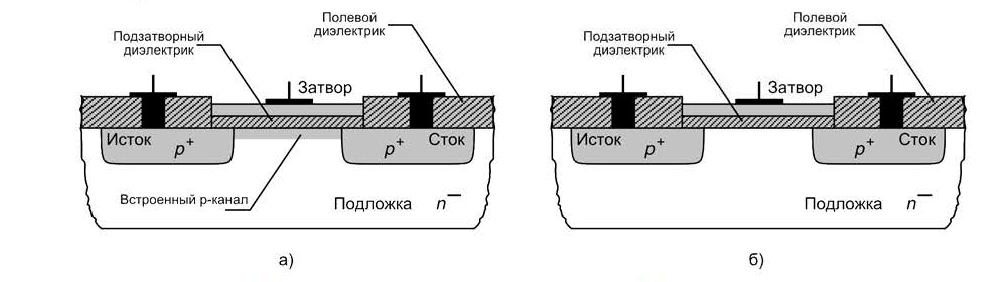
\includegraphics[width=\linewidth]{image/Teor_MOP_1}
	\caption{Структуры р-канальных МОП-транзисторов со встроенным (а) и индуцированным (6) каналами}
	\label{fig:teormop1}
\end{figure}

\begin{figure}
	\centering
	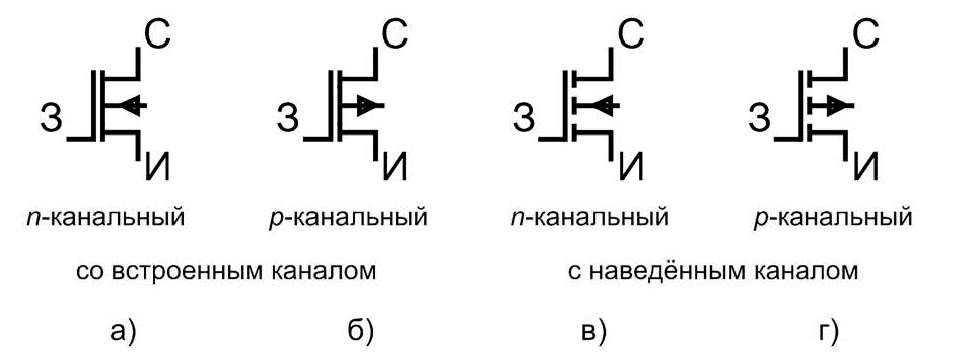
\includegraphics[width=0.7\linewidth]{image/Teor_MOP_2}
	\caption{Обозначения МОПТ на электрических схемах}
	\label{fig:teormop2}
\end{figure}

\subsection{Принцип действия МОПТ}

Принцип действия МОПТ с наведённым каналом. Работа МОПТ
определяется в основном двумя управляющими напряжениями: затвора
и стока, которые обычно отсчитываются относительно потенциала истока:
Vзи, Vси (\imref{fig:teormop3}).
При изменении напряжения затвора Vзи формируется (или наоборот
перекрывается) проводящий канал. При Vзи = О канал отсутствует, ток в выходной
цепи равен обратному тепловому току р-n-переходов.
При повышении Vзи сначала образуется обеднённый слой ( объёмный заряд
ионов: акцепторов в случае n-МОПТ и доноров в случае р-МОПТ),
 а затем - при напряжении затвора Vзи = $Vpor$, называемом пороговым,
- инверсионный слой электронов, который как раз и является проводящим
каналом. Свободные носители заряда, составляющие канал,
притягиваются электрическим полем затвора частично из области подложки,
но большей частью из областей стока и истока. На сток-затворной
( ещё говорят: передаточной, или проходной 1 ) вольт-амперной характеристике
Jс(Vзи) значение Vзи = Vпор разделяет два участка (\imref{fig:teormop5} а) . Согласно
физическому определению, пороговым напряжением затвора называется такое,
при котором концентрация свободных электронов в тонком приповерхностном
слое становится равной исходной концентрации свободных дырок в
объёме подложки. При Vзи > Vпор транзистор условно считается открытым.
При изменении напряжения стока меняется форма канала. При Vси > О
потенциал в канале является неравномерным: вблизи истока (х = О, если отсчитывать
от начала канала) он определяется практически только полем затвора
и равен Vзи - Vпор, а вблизи стока (х = L, где L - длина затвора) совместным
действием полей затвора и стока и равен Vзи - f!;.юр - Vси. Соответственно,
с увеличением Vси толщина канала со стороны стока уменьшается.
 При достижении напряжением стока некоторого критического
значения, называемого напряжением насыщения: Vси,нас = Vзи - Vпор, сечение
канала вблизи стока в точке х = L уменьшается до О (это называется отсечкой
канала), так как напряжение между затвором и поверхностью полупроводника
в этой точке становится равным пороговому напряжению.
При дальнейшем увеличении напряжения стока Vси > Vси,нас фактическая
(«эффективная») длина канала LэФФ = L - ЛL становится меньше L
2, а оставшееся до области стока расстояние ЛL занимает расширившаяся
обеднённая область (ОПЗ) обратносмещённого стокового р-nперехода.
Проводимость транзистора обеспечивается следующим образом:
носители заряда, прошедшие из области истока к концу канала, подхватываются
сильным электрически полем стокового р-n-перехода и дрейфуют к области
стока. В итоге ток стока слабо увеличивается, график его
зависимости от напряжения стока имеет небольшой наклон. Геометрическое
место значений Vси,нас = Vзи - Vпор разделяет триодный (крутой) и пентодный
(пологий) участки на выходных характеристиках (\imref{fig:teormop4}).
Принцип действия МОПТ со встроенным каналом отличается тем,
что пороговое напряжение у такого прибора (называемое здесь напряжением
отсечки) имеет отрицательное значение, что влияет на вид его волыамперных
характеристик.

\begin{figure}
	\centering
	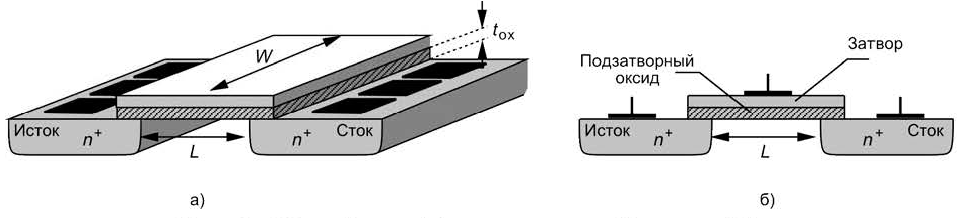
\includegraphics[width=\linewidth]{image/Teor_MOP_3}
	\caption{Общий вид (а) и продольный разрез (6) n-канального МОП-транзистора}
	\label{fig:teormop3}
\end{figure}

\begin{figure}
	\centering
	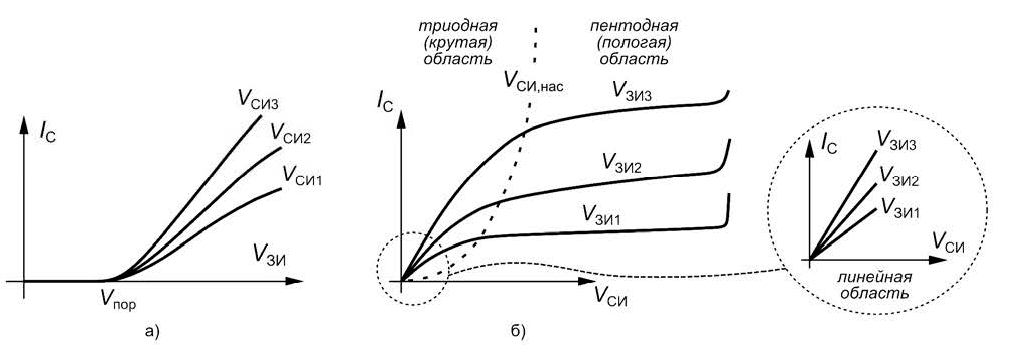
\includegraphics[width=\linewidth]{image/Teor_MOP_4}
	\caption{Вид сток-затворных Iс(Vзи) (а) и выходных Iс(Vси) (6) вольт- амперных характеристик МОПТ}
	\label{fig:teormop4}
\end{figure}

\section{Схемы измерений}

\section{Результаты измерений}
\subsection{Графики измерений}
\section{Вычисление параметров модели}
\section{Схемы расчета ВАХ}
\section{Графики ВАХ}
\end{document} % конец документа